\documentclass{standalone}
\author{Quinten Bruynseraede}
\usepackage{tikz}
\usetikzlibrary{shapes}
\title{Tikz grafen}
\begin{document}\pagestyle{empty}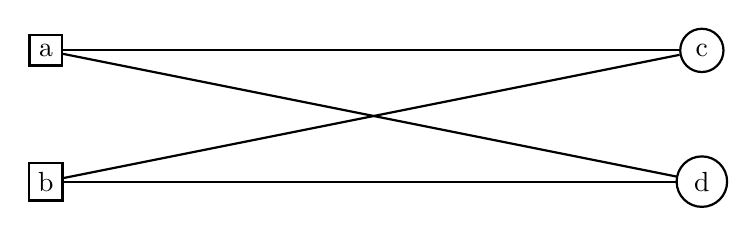
\begin{tikzpicture}\node[shape=rectangle,draw=black,align=center,line width=0.8pt] (0) at (1.6666666666666667,15.0) {a};
\node[shape=rectangle,draw=black,align=center,line width=0.8pt] (1) at (1.6666666666666667,13.333333333333334) {b};
\node[shape=circle,draw=black,align=center,line width=0.8pt] (2) at (10.0,15.0) {c};
\node[shape=circle,draw=black,align=center,line width=0.8pt] (3) at (10.0,13.333333333333334) {d};

\path [-,draw=black,line width=0.8pt] (0) edge node {} (2);
\path [-,draw=black,line width=0.8pt] (0) edge node {} (3);
\path [-,draw=black,line width=0.8pt] (1) edge node {} (2);
\path [-,draw=black,line width=0.8pt] (1) edge node {} (3);
\end{tikzpicture}
\end{document}